\section{Bayesian Networks}
\subsection{Basic concepts}
A Bayesian network ($G, P$) consists of:\\
- A BN structure $G$ (directed, acyclic graph)\\
- A set of conditional probability distributions\\
- ($G, P$) defines the joint distribution:\\
    $P(X_1, ..., X_n)=\prod_iP(X_i | Pa_{X_i})$

BNs with 3 nodes:

% 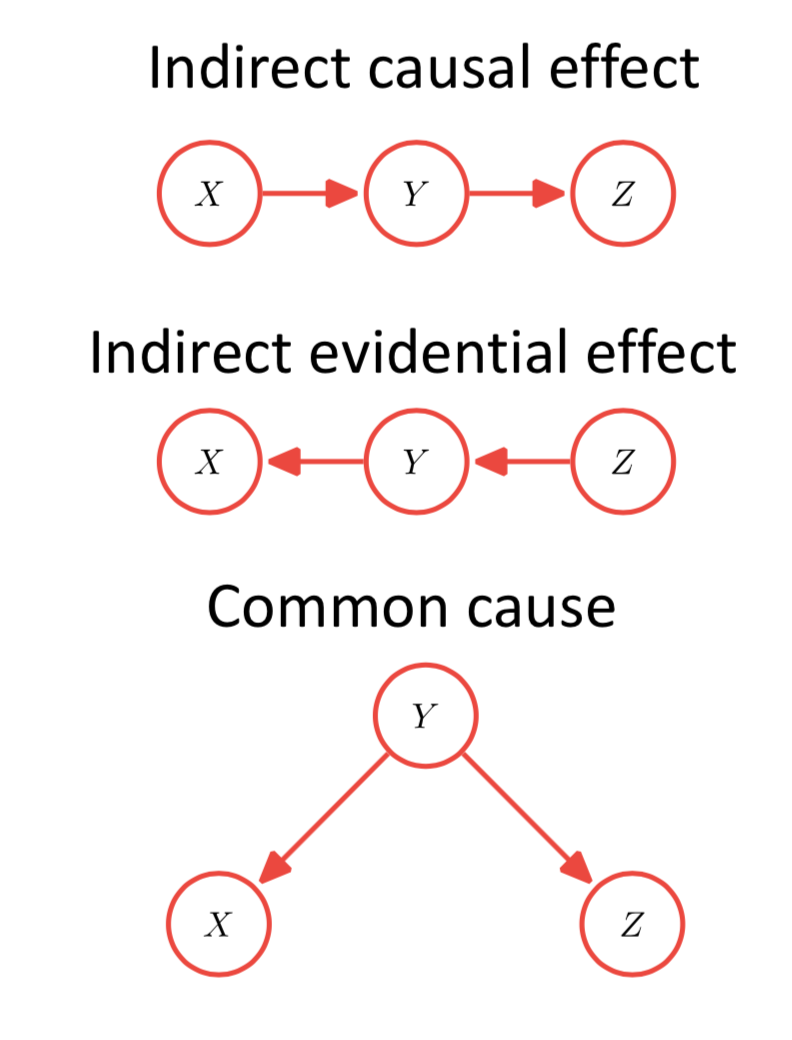
\includegraphics[scale=.2]{BN1.png}
% 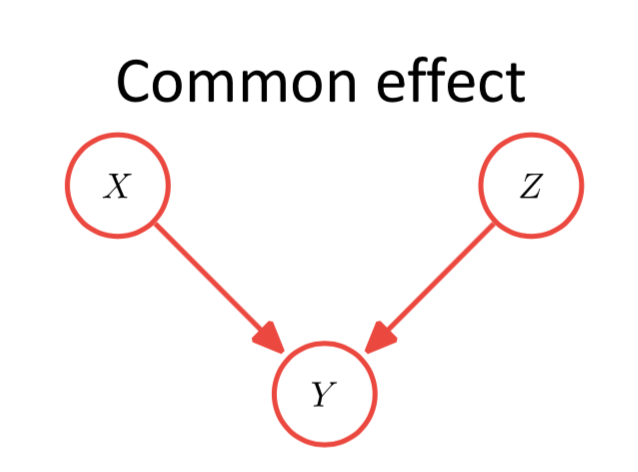
\includegraphics[scale=.2]{BN2.png}
\subsection{Active trails and d-separation}
An undirected path in a BN structure G is called active trail for observed variables $O \in {X_1, ..., X_n}$ of for every consecutive triple of variables X, Y, Z on the path:\\
- \textbf{indirect causal effect}:\\
$X \rightarrow Y \rightarrow Z$ and Y unobserved\\
- \textbf{indirect evidential effect}:\\
$X \leftarrow Y \leftarrow Z$ and Y unobserved\\
- \textbf{common cause}:\\
$X \leftarrow Y \rightarrow Z$ and Y unobserved.\\
- \textbf{common effect}:\\
$X \rightarrow Y \leftarrow Z$ and Y or any of Y's descendants is observed.\\
Any variables $X_i$ and $X_j$ for which there is no active trail for observations O are called d-separated by O.\\
\textbf{Theorem}: $d-sep(X_i;X_j|O)) \quad \Rightarrow X\perp Y |Z$\\
Converse does not hold in general!

